\chapter{आनुवंशिकता और लक्षण}\label{ch:g9:heredity-and-traits}

परिवार की तस्वीरें जीव विज्ञान के आँकड़े हैं। नन्हे बच्चे पर दादी की
ठुड्डी, माँ के घुँघराले बाल किसी भी बच्चे पर नहीं, एक भाई लंबा और एक
नहीं --- परिवारों में समानता चलती है, और फ़र्क़ भी। यह किताब बरसों से इस
तथ्य का सहारा लेती आई है (\cref{rem:g4:animal-reproduction:mix} वाला
बछेड़ा, \cref{prop:g8:sexual-reproduction:shuffle} वाले भाई-बहन); और इस
साल का पहला अध्याय आख़िरकार इसी का अध्ययन करता है: विरासत में मिलता
ठीक-ठीक क्या है, क्या नहीं मिलता, और परिवार की समानता के ढर्रे हमें क्या
नतीजा निकालने देते हैं।

\begin{omfigure}
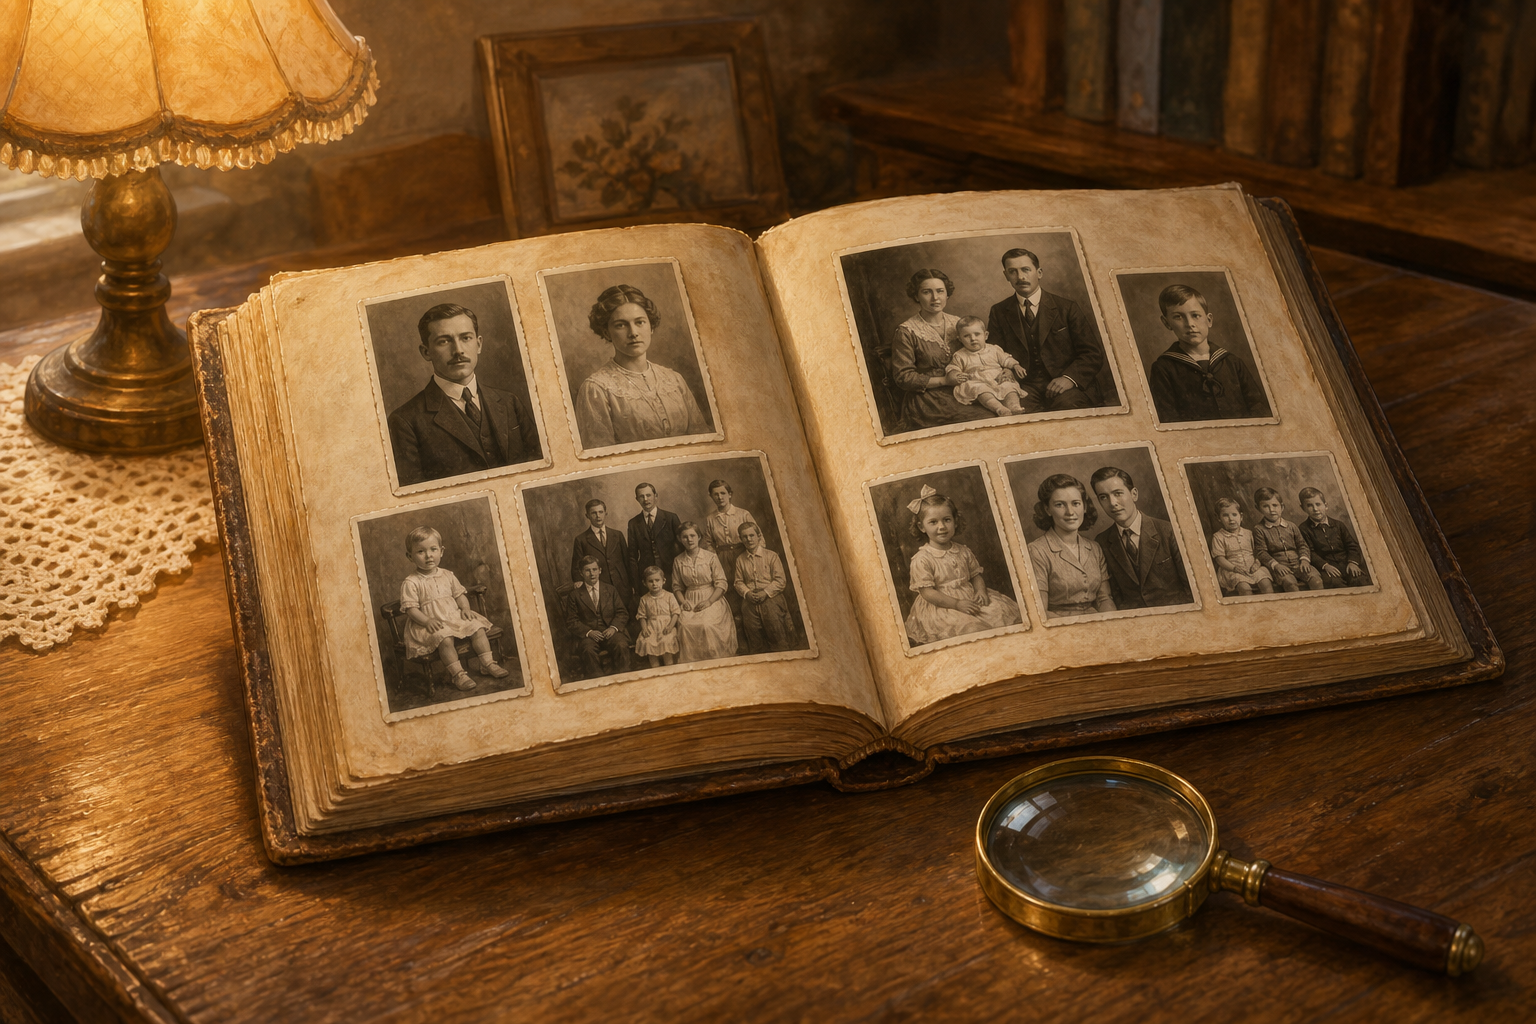
\includegraphics[width=0.62\linewidth]{images/book1/ai/g9-family-album.png}

{\small जीव विज्ञान के आँकड़े, सीपिया संस्करण में: पीढ़ी-दर-पीढ़ी उतरती
समानता और उतरता फ़र्क़।}
\end{omfigure}

\section{लक्षण, और वे आते कहाँ से हैं}

\begin{definition}[लक्षण]\label{def:g9:heredity-and-traits:traits}
\emph{लक्षण}\index{लक्षण} किसी व्यक्ति की कोई भी बताई जा सकने वाली
ख़ासियत है: \omterm{def:g1:the-five-senses:sense}{आँखों} का रंग, रक्त-समूह, \omterm{def:g1:the-five-senses:sense}{कान} की लौ की शक्ल, लंबाई, गाने वाली
आवाज़, कोई निशान। किसी व्यक्ति के लक्षणों का पूरा जमघट दो कारीगरियों से
बनता है: जो \emph{विरासत में मिला}, और जो \emph{\omterm{def:g6:exploring-our-environment:components}{पर्यावरण} तथा जीवन} ने
जोड़ा (\cref{def:g4:adapted-to-their-world:adaptation} वाली दुनिया, एक
ही शरीर पर काम करती हुई)।
\end{definition}

\begin{definition}[आनुवंशिकता]\label{def:g9:heredity-and-traits:heredity}
\emph{आनुवंशिकता}\index{आनुवंशिकता} जनकों से संतान तक, जनन के ज़रिए,
\omterm{def:g9:heredity-and-traits:traits}{लक्षणों} का पहुँचना है --- और जनन, जैसा
\cref{ch:g8:sexual-reproduction} ने दिखाया, दो अकेली \omterm{def:g5:first-look-at-cells:cell}{कोशिकाओं} से होकर
चलता है। जो \omterm{def:g9:heredity-and-traits:traits}{लक्षण} इस रास्ते से जाते हैं वे \emph{आनुवंशिक
लक्षण}\index{आनुवंशिक लक्षण} हैं: \omterm{def:g1:the-five-senses:sense}{आँखों} का रंग और रक्त-समूह हैं; और
निशान तथा छिदे हुए \omterm{def:g1:the-five-senses:sense}{कान} नहीं, चाहे कितने ही बरस पहने गए हों। छाँटने की
कसौटी \omterm{def:g8:sexual-reproduction:gametes}{युग्मक} हैं: जो दो \omterm{def:g5:first-look-at-cells:cell}{कोशिकाएँ} ढो नहीं सकतीं, परिवार वह पहुँचा नहीं
सकते।
\end{definition}

\begin{example}[परिवार का एलबम छाँटना]\label{ex:g9:heredity-and-traits:album}
दादा की तस्वीरें: उनकी वह ख़ास नाक --- आनुवंशिक, वह बुआ और चचेरे भाई पर
फिर हाज़िर है; उनकी धूप में पकी किसान वाली रंगत --- हासिल की हुई, और
दफ़्तर में काम करते उनके पोते के पास नहीं है; उनकी लंबाई --- कुछ हद तक
दोनों, क्योंकि उसी चौखट पर पोता उनसे ऊपर निकल जाता है, समृद्ध सालों का
खिलाया हुआ (\cref{prop:g3:balanced-diet:jobs}); और उनका वायलिन का हुनर
--- हुनर के तौर पर आनुवंशिक नहीं
(\cref{ex:g8:nervous-communication:juggler}: \omterm{def:g8:nervous-communication:synapse}{तंत्रिका-संधियाँ} सधती हैं,
पहुँचाई नहीं जातीं), हालाँकि वह संगीत वाला परिवार बताता है कि जो कुछ
आगे जाता है उसमें कुछ ज़्यादा सूक्ष्म भी काम कर रहा है: शायद रुझान,
सधे हुए तार ख़ुद कभी नहीं।
\end{example}

\begin{proposition}[विरासत में मिला और हासिल किया हुआ]\label{prop:g9:heredity-and-traits:sorting}
ये दोनों कारीगरियाँ तीन कसौटियों पर अलग हो जाती हैं:
\begin{enumerate}
  \item \emph{परिवार का ढर्रा}: \omterm{def:g9:heredity-and-traits:heredity}{आनुवंशिक लक्षण} वंश-वृक्ष में जनन की
        लकीरों के साथ-साथ लौटते हैं; और हासिल किए हुए \omterm{def:g9:heredity-and-traits:traits}{लक्षण} जीवन के
        पीछे चलते हैं (सारे मल्लाह धूप में पके हुए, चाहे उनके जनक कोई
        भी हों);
  \item \emph{शुरू से हाज़िर होना}: रक्त-समूह \omterm{def:g5:flower-to-fruit:steps}{निषेचन} पर ही तय हो जाता
        है; और वह रंगत तथा वह हुनर बाद में बनते हैं;
  \item \emph{पहुँचना}: जिनके अंग कट चुके हों उनके बच्चों के अंग
        सलामत होते हैं; और शरीर सौष्ठव वालों के बच्चे बिना प्रशिक्षण के
        ही शुरू करते हैं। हासिल किए हुए \omterm{def:g9:heredity-and-traits:traits}{लक्षण} अपने हासिल करने वाले के
        साथ ही मर जाते हैं --- \omterm{def:g8:sexual-reproduction:gametes}{युग्मक} उन्हें ढोते ही नहीं।
\end{enumerate}
ज़्यादातर दिखने वाले \omterm{def:g9:heredity-and-traits:traits}{लक्षण} --- लंबाई, गठन, यहाँ तक कि मिज़ाज भी ---
दोनों कारीगरियों से बुने होते हैं: विरासत में मिली एक सीमा-सी, और जीवन
से भरा हुआ उसका भीतर।
\end{proposition}
\admitted

\section{परिवार के ढर्रे पढ़ना}

\begin{example}[वे लक्षण जो पीढ़ी छोड़ देते हैं]\label{ex:g9:heredity-and-traits:skip}
कुछ ढर्रे पहली नज़र में उलझा देते हैं: भूरी \omterm{def:g1:the-five-senses:sense}{आँखों} वाले दो जनकों की नीली
\omterm{def:g1:the-five-senses:sense}{आँखों} वाली संतान; या दादी का कोई \omterm{def:g9:heredity-and-traits:traits}{लक्षण}, जो उनके किसी बच्चे में नहीं
दिखता पर किसी नाती-पोते में लौट आता है। पीढ़ी छोड़ना आम है, और वह एक भारी
नतीजा भी ढोता है: कोई जनक \emph{वह पहुँचा सकता है जो वह ख़ुद दिखाता
नहीं}। उस \omterm{def:g9:heredity-and-traits:traits}{लक्षण} के निर्देश एक पूरी पीढ़ी में छिपे-छिपे सफ़र कर गए ---
इसलिए विरासत में मिलता ख़ुद वह \omterm{def:g9:heredity-and-traits:traits}{लक्षण} नहीं, बल्कि वह चीज़ है जो उसे
\emph{तय} करती है, और जो बिना दिखे ढोई जा सकती है।
\end{example}

\begin{proposition}[ये ढर्रे हमसे कौन-से नतीजे निकलवाते हैं]\label{prop:g9:heredity-and-traits:conclusions}
तीन नतीजे, और हर एक किसी अवलोकन का ज़ोर दिया हुआ:
\begin{enumerate}
  \item चूँकि हासिल किए हुए \omterm{def:g9:heredity-and-traits:traits}{लक्षण} आगे नहीं जाते, इसलिए जो जाता है वह
        \emph{निर्धारक} ही होगा --- यानी \omterm{def:g9:heredity-and-traits:traits}{लक्षण} बनाने के निर्देश, ख़ुद
        \omterm{def:g9:heredity-and-traits:traits}{लक्षण} नहीं;
  \item चूँकि \omterm{def:g9:heredity-and-traits:traits}{लक्षण} पीढ़ियाँ छोड़ देते हैं, इसलिए निर्धारक \emph{बिना
        दिखे ढोए} जा सकते हैं: हर व्यक्ति अपने दिखाए हुए से ज़्यादा
        ढोता है;
  \item और चूँकि हर संतान दोनों जनकों से, दो \omterm{def:g8:sexual-reproduction:gametes}{युग्मकों} के ज़रिए, पाती है
        (\cref{prop:g8:sexual-reproduction:core}), इसलिए हर जनक अपने
        निर्धारकों में से एक \emph{चुनाव} देता है --- और वे चुनाव
        संतान-दर-संतान अलग होते हैं, वरना भाई-बहन एक-से होते
        (\cref{prop:g8:sexual-reproduction:shuffle} वाली फेंटाई, अब
        अपनी जगह पर: वह \emph{निर्धारकों की} फेंटाई है)।
\end{enumerate}
\end{proposition}
\admitted

\begin{remark}[यह जो सवाल खड़ा करता है]\label{rem:g9:heredity-and-traits:question}
परिवार के एलबम ने हमें एक शानदार सवाल में घेर लिया है। किसी \omterm{def:g8:reproductive-systems:male}{शुक्राणु} के
उस लगभग-कुछ-नहीं में (\cref{ex:g8:reproductive-systems:sperm} --- एक
कसकर बँधा \omterm{def:g6:cell-unit-of-life:parts}{केंद्रक} और एक पूँछ) किसी नाक, किसी रक्त-समूह, \omterm{def:g1:the-five-senses:sense}{आँखों} के किसी
रंग के निर्देश सफ़र करते हैं --- बिना दिखे ढोए जाने लायक़, आधों में चुने
जाने लायक़, और बढ़ते हुए शरीर के पढ़े जाने लायक़। \emph{वे हैं कहाँ, और
बने किस चीज़ से हैं?} \omterm{def:g8:reproductive-systems:male}{शुक्राणु} की शरीर-रचना जवाब की तरफ़ पहले ही इशारा कर
देती है: पिता जो कुछ भेजता है वह सब एक \omterm{def:g6:cell-unit-of-life:parts}{केंद्रक} में समा जाता है
(\cref{rem:g5:first-look-at-cells:nucleus} ने वादा किया था कि यह जगह
मायने रखेगी)। अगले दो अध्याय उसे खोलते हैं।
\end{remark}

\begin{method}[किसी लक्षण की जाँच-पड़ताल]\label{met:g9:heredity-and-traits:audit}
किसी भी \omterm{def:g9:heredity-and-traits:traits}{लक्षण} के लिए ये तीनों कसौटियाँ चलाओ:
\begin{enumerate}
  \item उसे वंश-वृक्ष पर रखो: क्या वह जनन की लकीरों के पीछे चलता है,
        या जीवन और आदतों के?
  \item उसकी तारीख़ बताओ: शुरू से तय, या रास्ते में बना?
  \item \omterm{def:g8:sexual-reproduction:gametes}{युग्मक} वाली कसौटी लगाओ: क्या दो \omterm{def:g5:first-look-at-cells:cell}{कोशिकाएँ} उसे ढो सकती थीं?
        (कोई निशान नहीं ढो सकता; कोई रक्त-समूह ढो सकता है);
  \item और फ़ैसला: विरासत में मिला, हासिल किया हुआ, या --- और यही सबसे
        आम है --- विरासत में मिली एक सीमा, जिसे जीवन ने भरा।
\end{enumerate}
\end{method}

\section{अभ्यास}

\begin{exercise}[$\star$]\label{exo:g9:heredity-and-traits:1}
\omterm{def:g9:heredity-and-traits:traits}{लक्षण} और \omterm{def:g9:heredity-and-traits:heredity}{आनुवंशिकता} की परिभाषा दो, और छाँटने की कसौटी एक वाक्यांश में
बताओ।
\end{exercise}

\begin{exercise}[$\star$]\label{exo:g9:heredity-and-traits:2}
इन्हें छाँटो: रक्त-समूह; छिदा हुआ \omterm{def:g1:the-five-senses:sense}{कान}; झाइयाँ; फ़र्राटेदार फ़्रांसीसी;
\omterm{def:g1:the-five-senses:sense}{कान} की लौ की शक्ल।
\end{exercise}

\begin{exercise}[$\star$]\label{exo:g9:heredity-and-traits:3}
\cref{prop:g9:heredity-and-traits:sorting} की तीनों कसौटियाँ बताओ।
\end{exercise}

\begin{exercise}[$\star$]\label{exo:g9:heredity-and-traits:4}
शरीर सौष्ठव वालों के बच्चे बिना प्रशिक्षण के क्यों शुरू करते हैं? यह
क्या दिखाता है?
\end{exercise}

\begin{exercise}[$\star$]\label{exo:g9:heredity-and-traits:5}
पीढ़ी छोड़ता कोई \omterm{def:g9:heredity-and-traits:traits}{लक्षण} यह साबित करता है कि कोई जनक क्या कर सकता है?
\end{exercise}

\begin{exercise}[$\star$]\label{exo:g9:heredity-and-traits:6}
विरासत में \omterm{def:g9:heredity-and-traits:traits}{लक्षणों} के बजाय निर्धारक ही क्यों मिलने चाहिए? एक वाक्य में।
\end{exercise}

\begin{exercise}[$\star\star$]\label{exo:g9:heredity-and-traits:7}
उसी चौखट पर पोते की लंबाई ज़्यादा निकली। इस वाक्य में दोनों कारीगरियाँ
अलग-अलग करो।
\end{exercise}

\begin{exercise}[$\star\star$]\label{exo:g9:heredity-and-traits:8}
निर्धारकों की भाषा में समझाओ कि भाई-बहन अलग क्यों होते हैं --- और
समरूप जुड़वाँ (\cref{exo:g8:from-egg-to-birth:10}) क्यों नहीं।
\end{exercise}

\begin{exercise}[$\star\star$]\label{exo:g9:heredity-and-traits:9}
\cref{met:g9:heredity-and-traits:audit} इन पर चलाओ: (क) किसी परिवार में
बार-बार लौटता जल्दी सफ़ेद होता बाल; (ख) किसी फ़ुटबॉल खिलाड़ी का दमख़म।
\end{exercise}

\begin{exercise}[$\star\star$]\label{exo:g9:heredity-and-traits:10}
वायलिन वाला मामला: अगर सधा हुआ हुनर कभी नहीं जाता, तो वह संगीत वाला
परिवार क्या पहुँचा रहा हो सकता है? ध्यान से फ़र्क़ करो।
\end{exercise}

\begin{exercise}[$\star\star$]\label{exo:g9:heredity-and-traits:11}
भूरी \omterm{def:g1:the-five-senses:sense}{आँखों} वाले दो जनक, और नीली \omterm{def:g1:the-five-senses:sense}{आँखों} वाली संतान --- और पड़ोसी को उस
परिवार पर शक है। \cref{ex:g9:heredity-and-traits:skip} के तर्क से उस
परिवार का बचाव करो।
\end{exercise}

\begin{exercise}[$\star\star\star$]\label{exo:g9:heredity-and-traits:12}
अकेले \omterm{def:g8:reproductive-systems:male}{शुक्राणु} की शरीर-रचना से
(\cref{ex:g8:reproductive-systems:sperm}) दलील दो कि पिता के निर्धारक
कहाँ बैठे होने चाहिए --- और पूरे इंसान के निर्देशों के लिए इससे कौन-सा
आकार निकलता है।
\end{exercise}

\section{समस्या: गाँव का वंशावलीकार}

\begin{problem}[{सप्ताहांत समस्या --- तीन पीढ़ियाँ, और लक्षणों की एक
बही}]\label{pb:g9:heredity-and-traits:1}
एक गाँव का वंशावलीकार गिरजे के वंश-वृक्षों पर \omterm{def:g9:heredity-and-traits:traits}{लक्षणों} की टिप्पणियाँ
लिखता है: ``गिरजा-ठुड्डी'' (एक ख़ास ठुड्डी, जो सदी भर लौटती रही है),
बाएँ हाथ का इस्तेमाल, नानबाइयों की आटे वाली फेफड़ा-खाँसी, रक्तदान की बही
से रक्त-समूह, और गड़ेरियों के धूप में पके चेहरे।

\medskip\noindent\textbf{भाग I --- बही को छाँटना।}
\begin{enumerate}
  \item पाँचों \omterm{def:g9:heredity-and-traits:traits}{लक्षणों} को
        \cref{met:g9:heredity-and-traits:audit} से छाँटो, और हर एक के
        लिए फ़ैसला करने वाली कसौटी भी बताओ।
  \item वह खाँसी नानबाई-ख़ाने के पीछे चलती है, परिवार के नहीं: ब्याह
        कर आने वाले उसे पा लेते हैं, और वहाँ से चले जाने वाले गँवा
        देते हैं। यह कौन-सी कसौटी है, काम पर?
  \item गिरजा-ठुड्डी दो शाखाओं में बीच वाली पीढ़ी छोड़ देती है। इससे
        निकलने वाला नतीजा बताओ।
  \item रक्त-समूह कभी-कभी बही को चौंका देते हैं: A और B समूह वाले
        जनकों की O समूह वाली संतान। हर जनक ने क्या-क्या ढोया होगा?
\end{enumerate}

\medskip\noindent\textbf{भाग II --- निर्धारकों वाली पढ़त।}
\begin{enumerate}[resume]
  \item उस ठुड्डी की सदी को निर्धारकों की भाषा में फिर से लिखो: चार
        पीढ़ियों तक असल में सफ़र क्या करता रहा, और किन सवारियों में
        (\cref{def:g9:heredity-and-traits:heredity})?
  \item ठुड्डी वाले चचेरे भाई-बहन बाक़ी हर बात में अलग क्यों हैं?
        फेंटाई की जगह बताओ।
  \item वंशावलीकार को सदी भर में एक भी ऐसा मामला नहीं मिलता जिसमें कोई
        निशान, कोई पेशा या कोई भाषा किसी नवजात तक पहुँची हो। उस आम
        नियम को बताओ, और उसकी कार्य-प्रणाली के दर्जे वाली वजह भी।
  \item एक परिवार के जुड़वाँ ठुड्डी में और उससे आगे भी एक-से मिलते
        हैं। उनकी शुरुआत के बारे में यह बही क्या नतीजा निकालती है
        (\cref{rem:g5:human-reproduction:twins})?
\end{enumerate}

\medskip\noindent\textbf{भाग III --- व्याख्यान।}
\begin{enumerate}[resume]
  \item वंशावलीकार भाषण देता है: ``यह गिरजा-बस्ती दो विरासतें
        पहुँचाती है --- एक \omterm{def:g8:sexual-reproduction:gametes}{युग्मकों} से, और एक साथ-साथ रहने से।'' बही
        के पाँचों \omterm{def:g9:heredity-and-traits:traits}{लक्षणों} को इन दोनों रास्तों में बाँटो।
  \item ``हममें से हर कोई जितना ढोता है उससे कम दिखाता है।'' इसका बचाव
        बही से, दो बार करो।
  \item एक श्रोता पूछता है कि \omterm{def:g8:sexual-reproduction:gametes}{युग्मक} वाले रास्ते के निर्देश भौतिक रूप
        में हैं क्या। \cref{rem:g9:heredity-and-traits:question} वाला
        ईमानदार जवाब दो --- जगह मालूम है, और सामग्री अगले अध्याय की
        बात।
  \item भाषण का समापन सबसे आम मामले पर जाँच-पड़ताल के एक पंक्ति वाले
        फ़ैसले से करो: ज़्यादातर \omterm{def:g9:heredity-and-traits:traits}{लक्षण} \emph{क्या} हैं, और
        \emph{कैसे} जिए जाते हैं?
\end{enumerate}
\end{problem}
